\section{旋转运动学}

\begin{comment}
\end{comment}
\begin{frame}
\frametitle{旋转运动学 \hfill 
\includegraphics[height=0.5cm]{00_logo.png}}
\begin{columns}
  \column{0.1\textwidth}
  
	\column{0.5\textwidth}
	\begin{itemize}
		\item 粒子在坐标系中$z=h$中的平面做圆周运动,坐标为:$r=(a\cos\theta, a \sin \theta, h)^T$,对坐标求导得:

    \begin{equation}
      \begin{split}
        \dot{r} &= (-a \dot{\theta} \sin \theta, a\dot{\theta}\cos\theta, 0)^T \\ 
          &= \begin{bmatrix}
        0 & -\dot{\theta} & 0 \\
        \dot{\theta} & 0 & 0 \\
        0 & 0 & 0 \\
      \end{bmatrix}
      \begin{bmatrix}
        a\cos\theta \\ a\sin\theta \\ h
      \end{bmatrix} \\
      &= w^\land r
      \end{split}
    \end{equation}

    其中,$w^\land$是一个反对称矩阵,$w = (0, 0, \dot{\theta})$, $\dot{\theta}$是角速度.

    % \item 对上式公式两边取模得:  
    
    % \begin{equation}
    %   |\dot{r}| = |w| |r| \sin \phi = a|\dot{\theta}|
    % \end{equation}


  \end{itemize}
  
  \column{0.3\textwidth}
	\begin{figure}[h]
		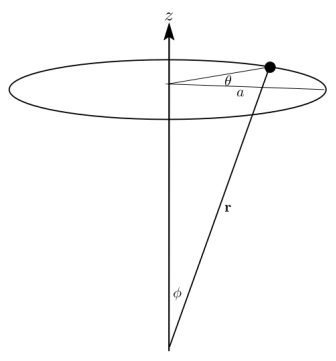
\includegraphics[trim=1.5 0 0 0, height=3.5cm,clip]{11_0.png}
		% \caption{四个区域搜索空间}
  \end{figure}
  
	\column{0.1\textwidth}

\end{columns}
\end{frame}

%%%%%%%%%%%%%%%%%%%%%%%%%%%%

\begin{frame}
  \frametitle{旋转运动学 \hfill 
\includegraphics[height=0.5cm]{00_logo.png}}
  \begin{columns}
    \column{0.1\textwidth}
    
    \column{0.8\textwidth}
    \begin{itemize}
      \item 旋转矩阵是一个行列式为1的正交矩阵.且每个列向量都是单位向量且相互正交,它的逆等于它的转置.
      % \item 旋转矩阵求导:
      % \begin{equation}
      %   \begin{split}
      %     \dot{R}(t)R(t)^T &= \phi(t)^\land \\
      %     \dot{R}(t) &= \phi(t)^\land R(t) \\
      %   \end{split}
      % \end{equation} 

      \item 旋转矩阵求导:
      \begin{equation}
        \begin{split}
          \dot{R}_{ib} &= \lim_{\Delta t \to 0} \frac{R_{ib} exp([w^b\Delta t]^\land) - R_{ib}}{\Delta t} \\
          &= \lim_{\Delta t \to 0} \frac{R_{ib} (exp([w^b\Delta t]^\land) - I)}{\Delta t} \\
          &\approx R_{ib} [w^b]^\land  \\
          & = [R_{ib}w^b]^\land R_{ib} \\
          & = [w^i]^\land R_{ib}
        \end{split}
      \end{equation} 

      \item 旋转矩阵求导2:
      \begin{equation}
        \begin{split}
          \dot{R}(t)R(t)^T &= \phi(t)^\land \\
          \dot{R}(t) &= \phi(t)^\land R(t) \\
        \end{split}
      \end{equation} 

    \end{itemize}


    % {\color{red}旋转矩阵是一个正交矩阵.它的行列式为1,且每个列向量都是单位向量且相互正交,它的逆等于它的转置.}
    
    \column{0.1\textwidth}
  
  \end{columns}
  \end{frame}   



%%%%%%%%%%%%%%%%%%%%%%%%%%%%

\begin{frame}
  \frametitle{旋转运动学 \hfill 
\includegraphics[height=0.5cm]{00_logo.png}}
  \begin{columns}
    \column{0.1\textwidth}
    \column{0.8\textwidth}
    更复杂一点的情况:一个旋转的水平光滑圆盘上,有一个光滑的小球,从圆心沿着半径向外运动.
    
    \begin{itemize}
      \item 从圆盘旋转坐标系来观察,小球轨迹如何?
      \item 从世界的坐标系来观察,小球轨迹如何?
      \item 科氏力,离心力,欧拉力?
      
    \end{itemize}

    \begin{figure}[h]
      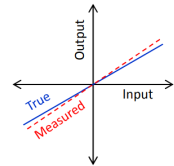
\includegraphics[trim=1.5 0 0 0, height=3.5cm,clip]{11_1.png}
      \qquad
      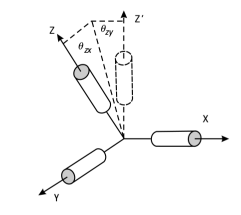
\includegraphics[trim=1.5 0 0 0, height=3.5cm,clip]{11_2.png}

      % \caption{四个区域搜索空间}
    \end{figure}
    \begin{figure}[h]
      % \caption{四个区域搜索空间}
    \end{figure}
    
    \column{0.1\textwidth}
  \end{columns}
  \end{frame}

%%%%%%%%%%%%%%%%%%%%%%%%%%%%

  \begin{frame}
    \frametitle{旋转运动学 \hfill 
\includegraphics[height=0.5cm]{00_logo.png}}
    \begin{columns}
      \column{0.1\textwidth}
      
      \column{0.5\textwidth}
      \begin{itemize}
        \item 质量块在body坐标系下的坐标为: $r^b = (x_1, x_2, x_3)^T$
        \item 忽略平移,只考虑旋转,旋转到惯性坐标系下:$r^i = R_{ib} r^b$
        \item 对时间求导:
    
        \begin{equation}
          \begin{split}
            \dot{r} &= R_{ib} \dot{r}^b + \dot{R}_{ib} r^b \\
            &= R_{ib} \dot{r}_b + R_{ib}[w^b]^\land r^b \\
            &= R_{ib} \dot{r}_b + [R_{ib}w^b]^\land R_{ib}r^b \\
            &= R_{ib} v^b + [w^i]^\land r^i \\
            &v = v^i + [w^i]^\land r^i  \Leftrightarrow
            v^i = v - [w^i]^\land r_i
          \end{split}
        \end{equation}
    
        其中,$w^i = R_{ib} w^b, v^i = R_{ib}v^b$, 表示body坐标系的角速度或线速度在I系下的表示.
    
    
      \end{itemize}
      
      \column{0.3\textwidth}
      \begin{figure}[h]
        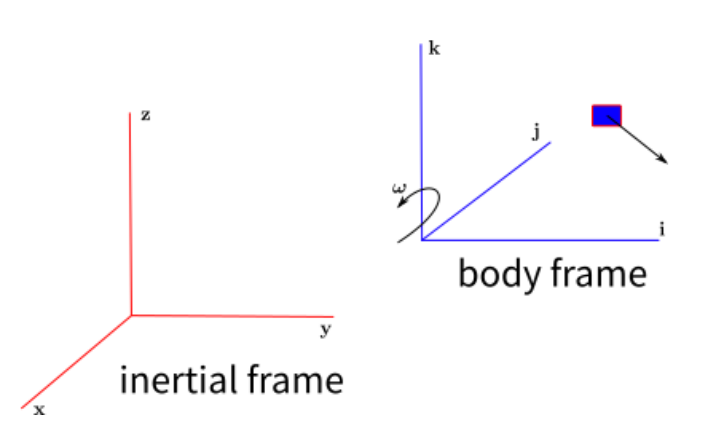
\includegraphics[trim=1.5 0 0 0, height=3.5cm,clip]{11_3.png}
        % \caption{四个区域搜索空间}
      \end{figure}
      
      \column{0.1\textwidth}
    
    \end{columns}
    \end{frame}  
  

   


  %%%%%%%%%%%%%%%%%%%%%%%%%%%%

\begin{frame}
  \frametitle{旋转运动学 \hfill 
\includegraphics[height=0.5cm]{00_logo.png}}
  \begin{columns}
    \column{0.1\textwidth}
    
    \column{0.8\textwidth}
    \begin{itemize}
      \item 对速度求导:
  
      \begin{equation}
        \begin{split}
          \ddot{r} &= R_{ib} \dot{v}^b + \dot{R}_{ib} v^b +  [w^i]^\land \dot{r}^i + [\dot{R}_{ib} w^b + R_{ib}\dot{w}^b]^\land r^i  \\ 
          &= R_{ib}\dot{v}^b + \dot{R}_{ib} v^b + [w^i]^\land \dot{r}^i +  [R_{ib}\dot{w}^b]^\land r^i  \\ 
          &= R_{ib} a^b + [w^i]^\land v^i + [w^i]^\land (v^i+[w^i]^\land r^i) + [\dot{w}^i]^\land r^i \\ 
          &= R_{ib} a^b + 2[w^i]^\land v^i + [w^i]^\land([w^i]^\land r^i) + [\dot{w}^i]^\land r^i \\
          \Rightarrow a^i &= a - \begin{matrix}
          \underbrace{2[w^i]^\land v^i}\\ Coriolis \ force
        \end{matrix} - \begin{matrix}
          \underbrace{[w^i]^\land([w^i]^\land r^i)}\\ centrifugal \ force
        \end{matrix} - \begin{matrix}
          \underbrace{[\dot{w}^i]^\land r^i}\\ Euler \ force 
        \end{matrix}
        \end{split}
      \end{equation}
  
      其中,$v^i = R_{ib}v^b, a^i = R_{ib}a^b$,表示物体在body下的速度或加速度在I系下的表示.

      
  
      {\color{red}在旋转坐标系下观察,运动的物体(运动方向和旋转轴不为同一个轴时)会受到科氏力的作用.}
    \end{itemize}
    
    \column{0.1\textwidth}
  
  \end{columns}
  \end{frame}      
  
  



